\documentclass[11pt]{article}

\usepackage{extras} % Se extras.sty
\usepackage{tikz}

\usetikzlibrary{positioning}
\usetikzlibrary{shapes}

\def\arraystretch{1.5}
\graphicspath{ {images/} }

\pagenumbering{roman}

\begin{document}
\begin{titlepage}
\begin{center}

{\Large\bfseries TSEA56 - Kandidatprojekt i elektronik \\ LIPS Kravspecifikation}

\vspace{5em}

Version 0.1

\vspace{5em}
%
Grupp 4 \\
\begin{tabular}{rl}
Hynén Ulfsjöö, Olle&\verb+ollul666+
\\
Wasteson, Emil&\verb+emiwa068+
\\
Tronje, Elena&\verb+eletr654+
\\
Gustafsson, Lovisa&\verb+lovgu777+
\\
Inge, Zimon&\verb+zimin415+
\\
Strömberg, Isak&\verb+isast763+
\\
\end{tabular}

\vspace{5em}
\today

\vspace{18em}
Status
\begin{longtable}{|l|l|l|} \hline

Granskad & - & - \\ \hline
Godkänd & - & - \\ \hline
 
\end{longtable}

\end{center}
\end{titlepage}

\pagebreak
\begin{center}

\section*{PROJEKTIDENTITET}
2016/VT, Undsättningsrobot Gr. 4

Linköpings tekniska högskola, ISY
\vspace{5em}
\begin{center}

\begin{tabular}{|l|l|l|l|} \hline
\textbf{Namn} & \textbf{Ansvar} & \textbf{Telefon} & \textbf{E-post}  \\ \hline 
Isak Strömberg & Projektledare & 073-980 38 50 & isast763@student.liu.se \\ \hline
Olle Hynén Ulfsjöö & - & 070-072 91 84 & ollul666@student.liu.se \\ \hline
Emil Wasteson & - & 076-836 61 66 & emiwa068@student.liu.se \\ \hline
Elena Tronje & - & 072-276 92 93 & eletr654@student.liu.se \\ \hline
Zimon Inge & - & 070-171 35 18 & zimin415@student.liu.se \\ \hline
Lovisa Gustafsson & - & 070-210 32 53 & lovgu777@student.liu.se \\ \hline
\end{tabular}

\end{center}

E-postlista för hela gruppen: isast763@student.liu.se

\vspace{5em}
Kund: ISY, Linköpings universitet
tel: 013-28 10 00, fax: 013-13 92 82, e-post: 
Kontaktperson hos kund:

\vspace{5em}
Kursansvarig:  \\
Handledare: 
\end{center}
\pagebreak

\tableofcontents

\pagebreak

\section*{Dokumenthistorik}
\begin{table}[h]
\begin{tabular}{|l|l|l|l|l|} \hline

\textbf{Version} & \textbf{Datum} & \textbf{Utförda förändringar} & \textbf{Utförda av} & \textbf{Granskad} \\ \hline
0.1 & 2016-01-25 &  Första utkastet & Grupp 4 & Nej \\ \hline
\end{tabular}
\end{table}

\pagebreak
\pagenumbering{arabic}

\begin{flushleft}

\section{Inledning}

Detta projekt har i uppgift att konstruera en robot. Innehållet i detta dokument specificerar vilken uppgift den fyller samt vilka krav som ställs på den.

\subsection{Parter}
I projektet finns följande parter:

\begin{itemize}
  \item \textbf{Beställare} av roboten är Mattias Krysander.
  \item \textbf{Handledare} från Linköpinngs universitet kommer att tilldelas vid senare tillfälle.
  \item \textbf{Expeter} finns att tillgå inom relevanta områden.
  \item \textbf{Projektgruppen} bestående av studenter vid I-programmet vid Linköpings universitet.
\end{itemize}

\subsection{Syfte och mål}
Syftet med projektet är att ta fram en första prototyp av en undsättningsrobot. 

Målsättningen är att roboten ska kunna genomföra sitt uppdrag.

\subsection{Användning}
Den färdiga roboten kommer att genomgå tester för att stämma av att kraven uppfyllts, samt en tävling mot robotar med samma projektdirektiv.

\subsection{Bakgrundsinformation}

Det finns ett intresse av att ta fram en robot som kan undersöka grottor och hjälpa nödställda. För att göra stor nytta ska den klara av okända områden och kunna beräkna kortaste vägen. 

\subsection{Definitioner}
Kraven listas enligt följade mall:

\begin{center}
\begin{longtable}{|l|l|p{.65\linewidth}|l|} \hline
Krav nr x & 
Status &
Beskrivning av krav x &
Prioritet \\ \hline
\end{longtable}
\end{center}

Varje krav har ett unikt nummer och en status, till exempel original och förändrat 2016-xx-xx. Beskrivningen visar vad som ska uppfyllas. Prioritet kan sättas i en tregradig skala enligt följande:


\pagebreak
\begin{itemize}
  \item Prioritet 1 är grundkrav, sådant som ska finnas med i den färdiga produkten.
  \item Prioritet 2 är krav som ska uppfyllas om det finns tid kvar då krav av prioritet 1 uppfyllts.
  \item Prioritet 3 är krav på framtida utbyggnad. Dessa uppfylls om det finns tid kvar då krav av prioritet 2 uppfyllts.
\end{itemize}


\pagebreak
\section{Översikt av systemet}

\begin{figure}[htbp]
\centering
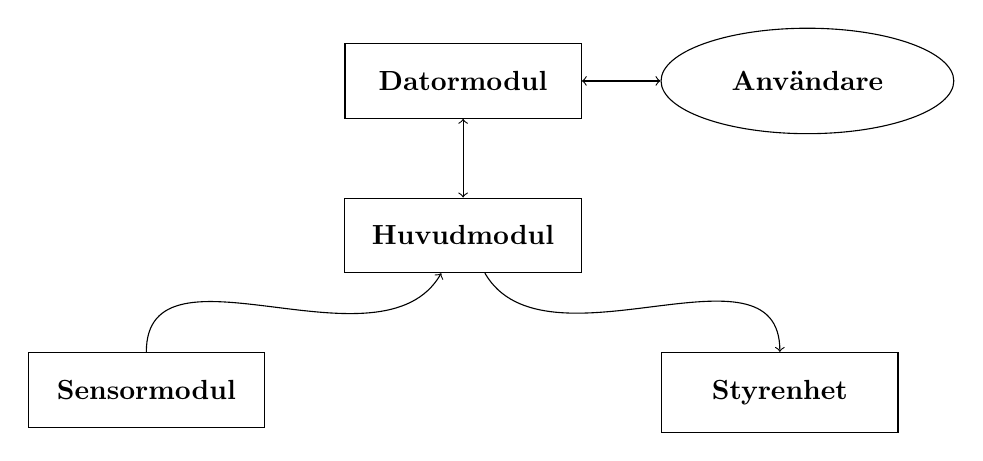
\begin{tikzpicture}[scale=1]
\tikzset{every node/.style={inner sep=10pt, minimum width=3 cm}}
%\draw[help lines,step=5mm,gray!20] (-5,-10) grid (5,0);
\node[draw, fill=white] (Huvudmodul)  {\textbf{Huvudmodul}};
\node[draw,below left= of Huvudmodul] (Sensormodul) {\textbf{Sensormodul}};
\node[draw,below right = of Huvudmodul] (Styrenhet) {\textbf{Styrenhet}};
\node[draw, above = of Huvudmodul] (Datormodul) {\textbf{Datormodul}};
\node[ellipse,draw, right = of Datormodul] (Användare) {\textbf{Användare}};

\draw[->] (Huvudmodul) [out=300, in= 90] to (Styrenhet);
\draw[->] (Sensormodul) [out=90, in=240] to (Huvudmodul);
\draw[<->] (Huvudmodul) to (Datormodul);
\draw[<->] (Datormodul) to (Användare);
\end{tikzpicture}
\caption{Överblick av systemet}
\end{figure}

\subsection{Grov beskrivning av produkten}

Roboten ska utifrån en definierad startpunkt utforska en okänd labyrint. Under den inledande rutten så skall mätdata från labyrinten samlas in och de nödställda i densamma skall identifieras. Den kortaste vägen mellan startpunkt och nödställda bestäms därefter varpå roboten återgår till sin startposition för att hämta förnödenheter. Roboten skall sedan navigera den kortaste vägen till de nödeställda för att avslutningsvis lämna förnödenheterna.

\subsection{Produktkomponenter}

Roboten skall internt bestå av tre komponenter:
\begin{itemize}
\item{En sensorkomponent vilken ska läsa av labyrinten samt bestämma avstånd och vinklar i densamma.} 
\item{En styrkomponent som sköter robotens drivlina och gripklo.}
\item{En huvudkomponent som kan kommunicera en karta av labyrinten till en extern datormodul samt mottaga kommandon från samma densamma. Huvudkomponenten skall därtill ge kommondon till styrkomponenten och kunna ta emot information från sensorkomponenten.}  
\end{itemize}  


\subsection{Beroenden till andra system}

Roboten ska med hälp av blåtand kunna kommunicera med en extern PC. Data ska kunna gå både från roboten till PC:n och vice versa.

\subsection{Ingående delsystem}
Roboten ska bestå av följande delsystem:
\begin{itemize}
	\item Huvudmodul som sköter alla beräkningar och all kommunikation
	\item Styrmodul som tar emot styrkommandon och kontrollerar robotens rörelser
	\item Sensormodul som tar emot data från robotens sensorer skickar vidare till huvudmodulen
\end{itemize}

\subsection{Avgränsningar}

\textit{vad ska det stå här?}

\subsection{Designfilosofi}
\textit{vad ska stå här?}

\subsection{Generella krav på hela systemet}
Nedan listas generella krav på hela systemet

\begin{center}
\begin{longtable}{|l|l|p{.65\linewidth}|l|} \hline

Krav nr\kravlista & 
Original & 
Roboten ska kunna navigera autonomt i en labyrint (designad enligt en given banspecifikation). & 
1 \\ \hline %Hur ska vi göra med dessa krav?

Krav nr\kravlista & 
Original & 
Roboten ska kunna kommunicera med en dator via blåtand& 
1 \\ \hline

\end{longtable}
\end{center}

\pagebreak
\section{Delsystem 1 - Huvudmodul}

\begin{figure}[htbp]
\centering
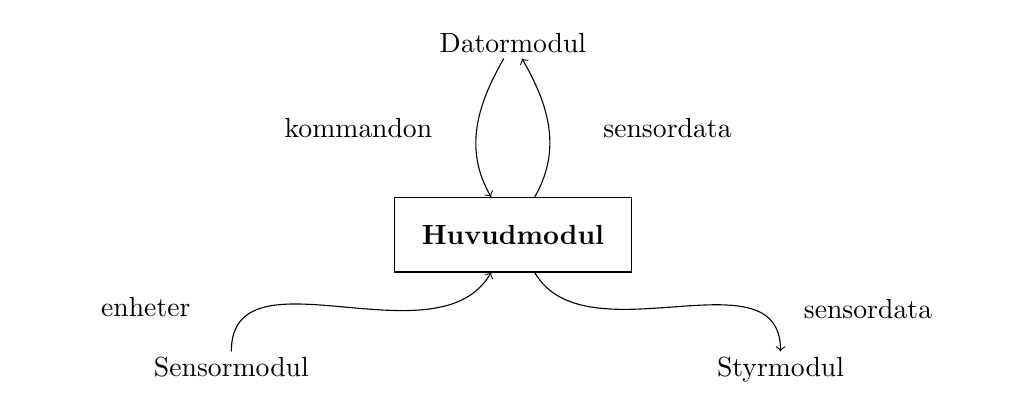
\begin{tikzpicture}[scale=1]
\tikzset{every node/.style={inner sep=10pt, minimum width=3 cm}}
%\draw[help lines,step=5mm,gray!20] (-5,-10) grid (5,0);

\node[draw] (Huvudmodul) {\textbf{Huvudmodul}};
\node[below left = of Huvudmodul,minimum width=0,inner sep=2pt] (Sensormodul) {Sensormodul};
\node[below right = of Huvudmodul, minimum width = 0, inner sep = 2pt] (Styrmodul) {Styrmodul};
\node[above = 5 em of Huvudmodul, minimum width = 0, inner sep = 2pt] (Datormodul) {Datormodul};

%\node[below right = of Styrmodul, minimum width = 0, inner sep = 2pt] (Motorer) {Motorer};
%\node[below left = of Styrmodul, minimum width = 0, inner sep= 2pt] (Gripklo) {Gripklo}


\draw[->] (Huvudmodul) [out=60,in=300] to node [midway, right] {sensordata} (Datormodul);
\draw[<-] (Huvudmodul) [out=120,in=240] to node [midway, left] {kommandon}  (Datormodul);

\draw[<-] (Huvudmodul) [out=240,in=90] to node [near end, left] {enheter} (Sensormodul);
\draw[->] (Huvudmodul) [out=300,in=90] to node [near end, right] {sensordata} (Styrmodul);

\end{tikzpicture}
\caption{Överblick av huvudmodul}
\end{figure}

\subsection{Inledande beskrivning av delsystem 1}
Delsystem 1 är robotens ``hjärna''. Här görs alla beräkningar kopplade till navigation i labyrinten och styrning av roboten. Denna del sköter även kommunikationen med en extern laptop genom blåtand.


\subsection{Gränssnitt}

\begin{center}
\begin{longtable}{|l|l|p{.65\linewidth}|l|} \hline

Krav nr\kravlista & 
Original &
Huvudmodulen ska kunna skicka styrkommandon till styrenheten. &
1 \\ \hline

Krav nr\kravlista & 
Original &
Huvudmodulen ska kunna ta emot mätadata från sensorenheten. &
1 \\ \hline

Krav nr\kravlista & 
Original &
Huvudmodulen ska kunna ta emot styrkommandon från dator via blåtand. &
1 \\ \hline

Krav nr\kravlista & 
Original &
Huvudmodulen ska kunna skicka mätdata till dator via blåtand. &
1 \\ \hline

\end{longtable}
\end{center}

\subsection{Designkrav}

\begin{center}
\begin{longtable}{|l|l|p{.65\linewidth}|l|} \hline

Krav nr\kravlista & 
Original &
Byte mellan autonomt och manuellt läge ska kunna göras med en brytare &
1 \\ \hline

Krav nr\kravlista & 
Original &
Tävlingsläge ska kunna initieras med en knapp &
1 \\ \hline

Krav nr\kravlista & 
Original &
Huvudmodulen ska kunna spela upp ljudsignaler &
2 \\ \hline

\end{longtable}
\end{center}

\subsection{Funktionella krav för delsystem 1}

\begin{center}
\begin{longtable}{|l|l|p{.65\linewidth}|l|} \hline

Krav nr\kravlista & 
Original &
Huvudmodulen ska kunna genomföra beräkningar för att hitta kortaste vägen givet en karta i en labyrint utan rum &
1 \\ \hline

Krav nr\kravlista & 
Original &
Huvudmodulen ska kunna genomföra beräkningar för att hitta kortaste vägen givet en karta i en labyrint med rum &
2 \\ \hline

Krav nr\kravlista & 
Original &
Huvudmodulen ska kunna reglera styrenheten så att roboten kör rakt i en labyrint utan rum &
1 \\ \hline

Krav nr\kravlista & 
Original &
Huvudmodulen ska kunna reglera styrenheten så att roboten kör rakt i en labyrint med rum &
2 \\ \hline

Krav nr\kravlista & 
Original &
Huvudmodulen ska kunna skicka styrkommandon till styrenheten &
1 \\ \hline

Krav nr\kravlista & 
Original &
Huvudmodulen ska kunna göra en kalibrering av sensorenheten &
1 \\ \hline

Krav nr\kravlista & 
Original &
Huvudmodulen ska kunna kalibrera styrenheten &
1 \\ \hline

Krav nr\kravlista & 
Original &
text text &
1 \\ \hline

\end{longtable}
\end{center}

\pagebreak
\section{Delsystem 2 - Sensormodul}

\begin{figure}[htbp]
\centering
\begin{tikzpicture}[scale=1]
\tikzset{every node/.style={inner sep=10pt, minimum width=3 cm}}
%\draw[help lines,step=5mm,gray!20] (-5,-10) grid (5,0);

\node[draw] (Sensormodul) {\textbf{Sensormodul}};
\node[above right = of Sensormodul,minimum width=0,inner sep=2pt] (Huvudmodul) {Huvudmodul};

\node[below left = of Sensormodul, minimum width = 0, inner sep = 2pt] (Sensor) {Sensorer};


\draw[->] (Sensor) [out=0,in=270] to node [sloped, midway, below] {spänningsnivåer} (Sensormodul);
\draw[->] (Sensormodul) [out=90,in=180] to node [sloped,midway, above] {enheter}  (Huvudmodul);

\end{tikzpicture}
\caption{Överblick av sensormodul}
\end{figure}

\subsection{Inledande beskrivning av delsystem 2}
Modulen samlar upp information från samtliga sensorer och konverterar respektive analogt mätvärde till en SI-enhet. Data skickas till huvudmodulen (delsystem 1) seriellt och ska även kunna presenteras på en display.

\begin{center}
\begin{longtable}{|l|l|p{.65\linewidth}|l|} \hline

Krav nr\kravlista & 
Original &
Sensormodulen ska samla in data från samtliga sensorer. &
1 \\ \hline



\end{longtable}
\end{center}

\subsection{Gränssnitt}

\begin{center}
\begin{longtable}{|l|l|p{.65\linewidth}|l|} \hline

Krav nr\kravlista & 
Original &
Sensormodulen ska seriellt skicka mätdata till huvudmodulen. &
1 \\ \hline


\end{longtable}
\end{center}

\subsection{Designkrav}

\begin{center}
\begin{longtable}{|l|l|p{.65\linewidth}|l|} \hline

Krav nr\kravlista & 
Original &
Sensormodulen ska presentera utgående data på en display. &
1 \\ \hline

\end{longtable}
\end{center}

\subsection{Funktionella krav för delsystem 2}

\begin{center}
\begin{longtable}{|l|l|p{.65\linewidth}|l|} \hline

Krav nr\kravlista & 
Original &
Sensormodulen ska konvertera sensorers mätdata till SI-enheter. &
1 \\ \hline



\end{longtable}
\end{center}

\pagebreak

\section{Delsystem 3 - Styrmodul}

\begin{figure}[htbp]
\centering
\begin{tikzpicture}[scale=1]
\tikzset{every node/.style={inner sep=10pt, minimum width=3 cm}}
%\draw[help lines,step=5mm,gray!20] (-5,-10) grid (5,0);

\node[draw] (Styrmodul) {\textbf{Styrmodul}};
\node[above left = of Styrmodul,minimum width=0,inner sep=2pt] (Huvudmodul) {Huvudmodul};

\node[below right = of Styrmodul, minimum width = 0, inner sep = 2pt] (Motorer) {Motorer};
%\node[below left = of Styrmodul, minimum width = 0, inner sep= 2pt] (Gripklo) {Gripklo}


\draw[->] (Styrmodul) [out=270,in=180] to node [sloped, midway, below] {spänningsnivåer} (Motorer);
\draw[<-] (Sensormodul) [out=90,in=0] to node [sloped,midway, above] {kommandon}  (Huvudmodul);

\end{tikzpicture}
\caption{Överblick av styrmodul}
\end{figure}

\subsection{Ska beskriva styrsystemet}
Styrmodulen ska kunna ta emot kommandon (kontinuerligt) från huvudmodulen och utifrån dessa instruktioner styra robotens elektriska motorer. Inga beräkningar ska göra av denna modul och inte heller någon reglering.

\subsection{Gränssnitt}

\begin{center}
\begin{longtable}{|l|l|p{.65\linewidth}|l|} \hline

Krav nr\kravlista & 
Original &
Styrmodulen ska kunna ta emot styrkommandon från huvudmodulen &
1 \\ \hline

\end{longtable}
\end{center}

\subsection{Designkrav}

\begin{center}
\begin{longtable}{|l|l|p{.65\linewidth}|l|} \hline

Krav nr\kravlista & 
Original &
Styrmodulen ska kunna &
2 \\ \hline

\end{longtable}
\end{center}

\subsection{Funktionella krav för delsystem 3}

\begin{center}
\begin{longtable}{|l|l|p{.65\linewidth}|l|} \hline

Krav nr\kravlista & 
Original &
Styrmodulen ska kunna köra roboten rakt fram/bak &
1 \\ \hline

Krav nr\kravlista & 
Original &
Styrmodulen ska kunna få roboten att rotera &
1 \\ \hline

Krav nr\kravlista & 
Original &
Styrmodulen ska kunna köra roboten fram/bak och svänga &
1 \\ \hline

Krav nr\kravlista & 
Original &
Styrmodulen ska kunna öppna och stänga gripklon&
1 \\ \hline

\end{longtable}
\end{center}

\pagebreak
\section{Delsystem 4 - Datormodul}

\begin{figure}[htbp]
\centering
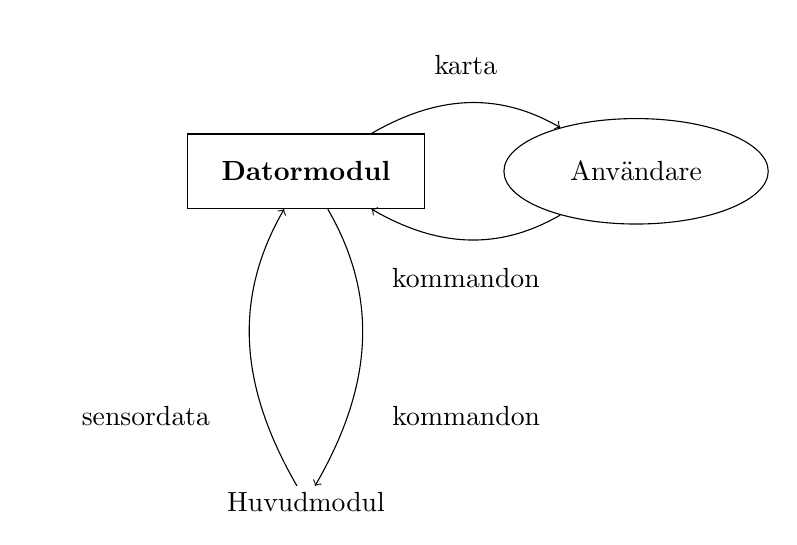
\begin{tikzpicture}[scale=1]
\tikzset{every node/.style={inner sep=10pt, minimum width=3 cm}}
%\draw[help lines,step=5mm,gray!20] (-5,-10) grid (5,0);

\node[draw] (Datormodul) {\textbf{Datormodul}};
\node[below = 10 em of Datormodul,minimum width=0,inner sep=2pt] (Huvudmodul) {Huvudmodul};
\node[right = of Datormodul, ellipse, draw] (Användare) {Användare};

%\node[below right = of Styrmodul, minimum width = 0, inner sep = 2pt] (Motorer) {Motorer};
%\node[below left = of Styrmodul, minimum width = 0, inner sep= 2pt] (Gripklo) {Gripklo}


\draw[->] (Datormodul) [out=30,in=150] to node [midway, above] {karta} (Användare);
\draw[<-] (Datormodul) [out=-30,in=210] to node [midway, below] {kommandon}  (Användare);

\draw[->] (Datormodul) [out=300,in=60] to node [near end, right] {kommandon} (Huvudmodul);
\draw[<-] (Datormodul) [out=240,in=120] to node [near end, left] {sensordata} (Huvudmodul);

\end{tikzpicture}
\caption{Överbilck av datormodul}
\end{figure}

\subsection{Inledande beskrivning av delsystem 4}

Datorprogram varan ska kunna rita upp en karta samt skicka styrkommandon till robotens huvudmodul.

\subsection{Gränssnitt}

\begin{center}
\begin{longtable}{|l|l|p{.65\linewidth}|l|} \hline

Krav nr\kravlista & 
Original &
Datormodulen ska kunna lista mätdata i en tabell &
1 \\ \hline

Krav nr\kravlista & 
Original &
Datormodulen ska kunna rita upp en 2D-karta &
2 \\ \hline

Krav nr\kravlista & 
Original &
Datormodulen ska kunna ta emot styrkommandon från användaren genom textinput &
1 \\ \hline

Krav nr\kravlista & 
Original &
Datormodulen ska kunna ta emot styrkommandon från användaren genom tangentbordsinput &
2 \\ \hline

\end{longtable}
\end{center}

\subsection{Designkrav}

\begin{center}
\begin{longtable}{|l|l|p{.65\linewidth}|l|} \hline

Krav nr\kravlista & 
Original &
Tabellen med mätdata ska presenteras på ett användarvänligt sätt &
1 \\ \hline

Krav nr\kravlista & 
Original &
2D-kartan ska ritas upp kontinuerligt allt eftersom ny mätdata erhålls &
2 \\ \hline

\end{longtable}
\end{center}

\subsection{Funktionella krav för delsystem 4}

\begin{center}
\begin{longtable}{|l|l|p{.65\linewidth}|l|} \hline

Krav nr\kravlista & 
Original &
Datorn ska kunna skicka styrkommandon till robotens huvudmodul via blåtand &
1 \\ \hline

\end{longtable}
\end{center}

\pagebreak
\section{Prestandakrav}

\begin{center}
\begin{longtable}{|l|l|p{.65\linewidth}|l|} \hline

Krav nr\kravlista &
Original &
\textit{vad ska det stå här?}&
2 \\ \hline

\end{longtable}
\end{center}

\section{Krav på vidareutveckling}

\begin{center}
\begin{longtable}{|l|l|p{.65\linewidth}|l|} \hline

Krav nr\kravlista &
Original &
\textit{vad ska det stå här?}&
1 \\ \hline

\end{longtable}
\end{center}

\section{Tillförlitlighet}

\begin{center}
\begin{longtable}{|l|l|p{.65\linewidth}|l|} \hline

Krav nr\kravlista &
Original &
\textit{vad ska det stå här?}&
1 \\ \hline

\end{longtable}
\end{center}

\section{Ekonomi}

\begin{center}
\begin{longtable}{|l|l|p{.65\linewidth}|l|} \hline

Krav nr\kravlista &
Original &
Projekt gruppen ska lägga 230 h/person &
1 \\ \hline
\end{longtable}
\end{center}

\section{Krav på säkerhet}

\begin{center}
\begin{longtable}{|l|l|p{.65\linewidth}|l|} \hline

Krav nr\kravlista &
Original &
\textit{vad ska det stå här?}&
1 \\ \hline

\end{longtable}
\end{center}

\pagebreak
\section{Leveranskrav och delleveranser}

\begin{center}
\begin{longtable}{|p{.01\linewidth} p{.07\linewidth} | p{.7\linewidth} | p{.1\linewidth} |} \hline
\textbf{Datum} & & \textbf{Aktivitet} & \textbf{BP} \\ \hline
22 & jan & Projektgruppen ska vara formad och projektuppgift vara vald. & BP0 \\ \hline
2 & feb & Kravspecifikationen ska vara klar. & BP1 \\ \hline
9 & feb & Val av förstudier ska vara inlämnade till beställaren. & - \\ \hline
15 & feb & Första versionen av projektplan, tidplan och systemskiss ska vara inlämnade till beställaren. & - \\ \hline
19 & feb & Slutgiltlig version av projektplan, tidplan och systemskiss ska vara inlämnade till beställaren.& BP2 \\ \hline
3 & mar & Första versionen av förstudien ska vara inlämnad till handledaren och beställaren. & - \\ \hline
11 & mar & Första versionen av designspecifikationen ska vara inlämnad till handledaren. & - \\ \hline
5 & apr & Designspecifikationen ska vara godkänd av handledaren. & BP3 \\ \hline
8 & apr & Version 1.0 av förstudien ska vara inlämnad till handledaren och beställaren. & - \\ \hline
15 & apr & Design ska vara presenterad och godkänd av handledaren. & BP4 \\ \hline
19 & maj & Version 1.0 av \textit{Kappan} (exklusive appendix) ska vara inlämnad. & - \\ \hline
25 & maj & Kraven ska vara verifierade.  & BP5 \\ \hline
26 & maj & Version 1.0 av teknisk dokumentation och användarhandledning ska vara inlämnade till beställaren. & - \\ \hline
\multicolumn{2}{| l |}{vecka  22} &  Redovisning och demostration. & - \\ \hline
3 & jun & Efterstudie och källskod ska vara inlämnade. & - \\ \hline
10 & jun & All utrsutning och nycklas ska vara återlämnade. & - \\ \hline
\end{longtable}
\end{center}

Utöver ovanstående leveranser ska tidsrapporter lämnas senaste kl 16.00 vid följande datum: 3 februari, 22 februari, 7 mars, 14 mars, 4 april, 11 april, 18 april, 25 april, 2 maj, 9 maj, 16 maj, 23 maj, 30 maj och 7 juni. 

\begin{center}
\begin{longtable}{|l|l|p{.65\linewidth}|l|} \hline

Krav nr\kravlista &
Original &
Alla leveranser och delleveranser ska lämnas in i tid.&
1 \\ \hline

\end{longtable}
\end{center}

\pagebreak
\section{Dokumentation}

\begin{center}
\begin{longtable}{|p{.18\linewidth}|p{.08\linewidth}|p{.35\linewidth}|p{.15\linewidth}|p{.09\linewidth}|}\hline
\textbf{Dokument} & \textbf{Språk} & \textbf{Syfte} & \textbf{Målgrupp} & \textbf{Format} \\ \hline

Kravspecifikation & SE & \textit{Listar de krav som ställs på slutprodukten.} & Projektgrupp och beställare & .pdf \\ \hline
Förstudie & SE & \textit{Utforska de tekniska alternativ som finns tillgängliga.} & Projektgrupp & .pdf \\ \hline
Projektplan & SE & \textit{Specificerar projektet upplägg.} & Projektgrupp & .pdf \\ \hline
Tidplan & SE & \textit{Planerar arbetsinsatsen.} & Projektgrupp & .pdf \\ \hline
Systemskiss & SE & \textit{Beskriver produktens upplägg.} & Projektgrupp & .pdf \\ \hline
Design-specifikation & SE & \textit{Ger en mer detaljerad specifikation av produkten.} & Projektgrupp & .pdf \\ \hline
Kappa & SE & \textit{Sammanfattar projektet.} & Beställare & .pdf \\ \hline
Teknisk- dokumentation & SE & \textit{Beskriver tekniken bakom produkten.} & Beställare & .pdf \\ \hline
Användar-handledning & SE & \textit{Beskriver hur produkten används.} & Beställare & .pdf \\ \hline
Efterstudie & SE & \textit{Reflekterar över projektet.} &Projektgrupp & .pdf \\ \hline
\end{longtable}
\end{center}

\section{Utbildning}

\begin{center}
\begin{longtable}{|l|l|p{.65\linewidth}|l|} \hline

Krav nr\kravlista &
Original &
\textit{vad ska det stå här?}&
1 \\ \hline

\end{longtable}
\end{center}

\section{Kvalitetskrav}

\begin{center}
\begin{longtable}{|l|l|p{.65\linewidth}|l|} \hline

Krav nr\kravlista &
Original &
\textit{vad ska det stå här?}&
1 \\ \hline

\end{longtable}
\end{center}

\section{Underhållsbarhet}

\begin{center}
\begin{longtable}{|l|l|p{.65\linewidth}|l|} \hline

Krav nr\kravlista &
Original &
\textit{vad ska det stå här?}&
1 \\ \hline

\end{longtable}
\end{center}

\pagebreak
\section{Referenser}

\begin{thebibliography}{9}
\bibitem{tidsplan}
ISY,
\emph{Leveranser i projektet 2016},
\url{http://www.isy.liu.se/edu/kurs/TSEA56/leveranser.html}
	
\end{thebibliography}



\end{flushleft}




\end{document}

